\section{Results}
Classification performances measured in local hold-out testing are presented for each of the methods are presented in Table \ref{tab:results}. Precision, recall and accuracy were computed on a hold-out split where 2.4 million examples were used for training, and the remaining 100 thousand samples were evaluated for testing.

\begin{table}[h]
  \centering
  \begin{tabular}[c]{lllll}
    Input format&Model&Accuracy&Precision&Recall\\
    \hline
    Tweet-embed.&Logistic regression & 60.60 &    60.84   & 60.64  \\
    Tweet-embed.&SVM             & 61.96    &   63.69     & 62.05   \\
    Tweet-embed.&Neural network & 65.45	& 67.04	& 65.53	 \\
    Word-embed.&CNN w/o dropout &  81.12  & 81.80	& 81.75	 \\
    Word-embed.&CNN w/ dropout & 84.29 & 84.79 & 84.74

  \end{tabular}
  \caption{Classification performances using local hold-out testing, for various input data formats. Reported values are percentages.}
  \label{tab:results}
\end{table}

Initial exploration of classification performances indicated that the neural network models would provide better results than the simpler linear classifiers. For this reason, we chose to train these models for a greater number of epochs. The classification performance of two convolutional neural networks over successive training epochs can be seen in Figure \ref{plot:CNNaccuracy}. During the training process, the hold-out data was classified at the end of each epoch, and its performance was reported, allowing us to track improvements in classification performance over time.

\label{sec:results}
\begin{figure}[h!]
  \centering
  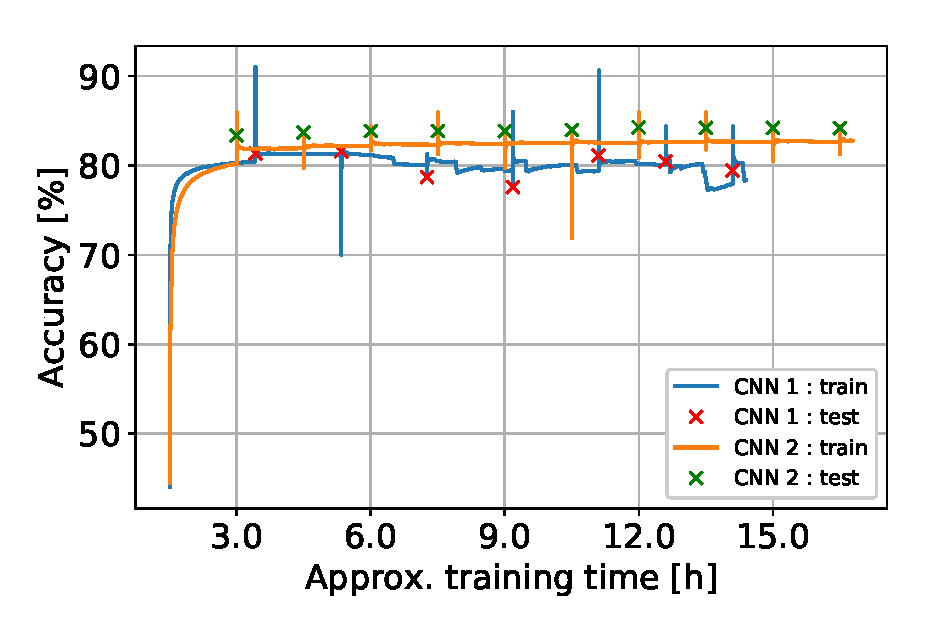
\includegraphics[scale=0.45]{CNNaccuracy}
  \caption{Hold-out classification accuracy over successive training epochs for two convolutional neural networks: CNN1 is a standard CNN, whereas CNN2 contains a dropout layer. Spikes in accuracy are caused by abberant values reported at the beginning of new epochs (indicated by crosses).}
  \label{plot:CNNaccuracy}
\end{figure}
\FloatBarrier

As expected, the convolutional network with a dropout layer was faster to train than without, allowing the model to be trained for further epochs. Furthermore, the regularizationinduced by the dropout layer yielded more accurate predictions. Extending the training time increased classification performance marginally, but naturally, perfomance plateaus at a certain point, after which additional training time has no benefit.
